%! Author = Sujal Singh
%! Date = 12/3/23

% Preamble
\documentclass[11pt]{beamer}
\title{Electrical Science Presentation}
\author[Aman, Ashish, Dhruv...]{\(|\) Aman Gupta \(|\) Ashish Chauhan \(|\) Dhruv Grover \(|\) Harsh Raj \(|\)\\
    \(|\) Pranav Bisht \(|\) Sujal Singh \(|\)}
\date[Harsh, Pranav, Sujal]{\textbf{Enrollment Numbers:\\}\texttt{0\{00,00,00,00,00,00\}00000000}}

\usetheme{Madrid}
\usecolortheme{spruce}
\setbeamertemplate{navigation symbols}{}
\setbeamertemplate{frametitle continuation}[from second][]

% Packages
\usepackage{amsmath}
\usepackage{lmodern}
\usepackage{siunitx}
\usepackage{tikz}
\usepackage[american]{circuitikz}

\usetikzlibrary{calc}
\ctikzset{voltage/american plus/.initial={}}
\ctikzset{voltage/american minus/.initial={}}
\makeatletter
\tikzset{cscale/.code={\pgf@circ@Rlen=#1\pgf@circ@Rlen},cscale/.default=1}
\makeatother

% Document
\begin{document}
    \begin{frame}{Electrical Science}
        \begin{center}
            %! suppress = FileNotFound
            
\includegraphics[width=80pt]{logo}
        \end{center}\vspace*{-10pt}
        \maketitle
    \end{frame}

    \begin{frame}[t]{Unit 2}
        \textbf{\large Explain the mathematical expression for voltage and current relationship in star and delta
        connection.}\\[10pt]

        \textbf{What are lines and phases?}

        The individual windings of a delta- or star-connected alternator or transformer, and their corresponding load
        impedance are called ``phases'', whereas the conductors that interconnect three-phase supplies and their loads
        are called ``lines'':\\[70pt]

        \begin{minipage}[c]{0.45\textwidth}
            \begin{circuitikz}[transform canvas={scale=0.8}]
                \draw (3,0) coordinate (C) node[below left] {\small $C$}
                to [inductor,l={\small phase},*-*] (6,0) coordinate (B) node[right] {\small $B$}
                (3,0) to [inductor,l={\small phase},-*] ++(60:3) coordinate (A) node[above] {\small $A$}
                to [inductor,l={\small phase}] ++(-60:3);

                \draw (A) to [short,-*] ++(-4,0) coordinate (a) node[left] {$A$};
                \draw (B) -- ++(0,-1) -- (C |- 0,-1) -- ++(-1,0) -- ++(0,2.3)
                to [short,-*] (a |- 0,1.3) coordinate (b) node[left] {$B$};
                \draw (C) to [short,-*] (a |- 0,0) coordinate (c) node[left] {$C$};

                \draw ($(a)+(1,0)$) node[above] {line};
                \draw ($(b)+(1,0)$) node[above] {line};
                \draw ($(c)+(1,0)$) node[above] {line};
            \end{circuitikz}
        \end{minipage}
        \begin{minipage}[c]{0.45\textwidth}
            \begin{circuitikz}[transform canvas={scale=0.8}]
                \draw (3,0) coordinate (C) node[below left] {\small $C$}
                to [cscale=0.6,inductor,l={\small phase},*-*] ++(1.5,1.29903) coordinate (O)
                to [cscale=0.6,inductor,l={\small phase},-*] ++(0,1.29903);
                \draw (O) to [cscale=0.6,inductor,l={\small phase},-*,invert] (6,0);

                \draw (A) to [short,-*] ++(-4,0) coordinate (a) node[left] {$A$};
                \draw (B) -- ++(0,-1) -- (C |- 0,-1) -- ++(-1,0) -- ++(0,2.3)
                to [short,-*] (a |- 0,1.3) coordinate (b) node[left] {$B$};
                \draw (C) to [short,-*] (a |- 0,0) coordinate (c) node[left] {$C$};

                \draw ($(a)+(1,0)$) node[above] {line};
                \draw ($(b)+(1,0)$) node[above] {line};
                \draw ($(c)+(1,0)$) node[above] {line};
            \end{circuitikz}
        \end{minipage}


    \end{frame}

    \begin{frame}[t,allowframebreaks]{Unit 3}
        \textbf{\Large Write the working principle of DC motor. Also explain the classification of different DC
        motors.}\\[20pt]

        \underline{\smash{\textbf{Flemming Left Hand Rule:}}}\\[10pt]
        If we stretch the first finger, second finger and thumb of our left hand to be perpendicular to each other,
        and first finger represents the direction of the magnetic field, the second finger represents the direction
        of the current, then the thumb represents the direction of the force experienced by the current carrying
        conductor.\\~\\

        \begin{center}
            \begin{tikzpicture}[transform canvas={scale=0.8}]
                \draw [->,red] (0,0) -- (0,1.5) node[above,red] {$\overrightarrow{F}$}
                \draw [->,blue] (0,0) -- (2,0.4) node[right,blue] {$\overrightarrow{B}$}
                \draw [->,green] (0,0) -- (2,-0.8) node[right,green] {$\overrightarrow{I}$}
            \end{tikzpicture}
        \end{center}

        \framebreak

        \underline{\smash{\textbf{Working Principle}}}\\[10pt]%

        \begin{center}
            \textit{``When a current carrying conductor is placed in a magnetic field, it experiences a mechanical
            force''}
        \end{center}

        A DC motor operates based on the principle of electromagnetic induction.\ It consists of a coil (armature)
        that carries current and is placed in a magnetic field.\ When current flows through the coil, it generates a
        magnetic field.\ The interaction between this magnetic field and the external magnetic field (created by
        stationary magnets or field windings) results in a torque, causing the motor to rotate.\ The commutator and
        brushes help to maintain the direction of current flow, ensuring continuous rotation.

        \framebreak

        \textbf{Diagram:}

        \begin{center}
            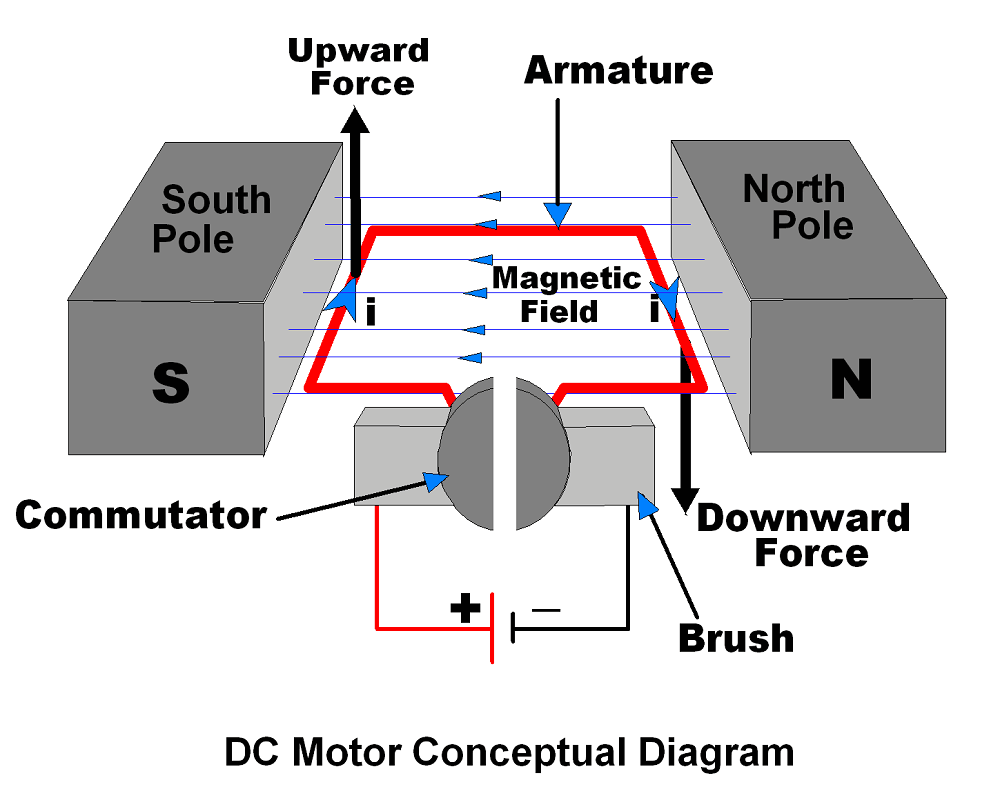
\includegraphics[width=200pt]{dc-motor-construction}
        \end{center}

        \framebreak

        \begin{center}
            \underline{\smash{\textbf{Types of DC Motor}}}\\[10pt]%
        \end{center}

        There are three types of motors:

        \begin{enumerate}
            \item Series Motor
            \item Shunt Motor
            \item Compound Motor
            \begin{enumerate}
                \item Long Shunt
                \item Short Shunt
            \end{enumerate}
        \end{enumerate}

        \framebreak

        \underline{\textbf{Series Motor:}}\\[10pt]%

        \begin{minipage}[c]{0.3\textwidth}
            $I_L = I_{se} = I_a$\vspace*{-10pt}
            \begin{flalign*}
                E_b + I_a R_a + I_{se} R_{se} - V_t &= 0\\
                E_b + I_a R_a + I_a R_{se} - V_t &= 0\\
                E_b + I_a \left( R_a + R_{se} \right) - V_t &= 0\\
            \end{flalign*}
            \vspace*{-35pt}
            \begin{center}
                $\boxed{V_t = E_b + T_a \left( R_a + R_{se} \right) + V_{\text{brush}}}$
            \end{center}
        \end{minipage}
        \begin{minipage}{0.14\textwidth}
            ~
        \end{minipage}
        \begin{minipage}[c]{0.45\textwidth}
            \begin{circuitikz}
                \draw (4,0) node[above right] {\small $-$} to (0,0)
                (0,4) to [R,l_=$R_a$] (0,2) to [V,i>_=$I_a$,l=$E_b$] (0,0)
                (0,4) [inductor,l=$R_{se}$,v=$I_{se}$] to (4,4) node[below right] {\small $+$};
                \draw [<->] (4,0.5) -- node[midway, right=5pt] {$V_t$} (4,3.5);
            \end{circuitikz}
        \end{minipage}

        \framebreak

        \underline{\textbf{Shunt Motor:}}\\[10pt]%

        \begin{minipage}[c]{0.3\textwidth}
            \begin{center}
                $I_L = I_{sh} + I_a$\\[10pt]
                $E_b + I_a R_a - V_t = 0$\\[10pt]
                $\boxed{V_t = E_b + I_a R_a}$\\[10pt]
                $\boxed{I_{sh} = \frac{V_t}{R_{sh}} = \frac{E_b + I_a R_a}{R_{sh}}}$
            \end{center}
        \end{minipage}
        \begin{minipage}{0.14\textwidth}
            ~
        \end{minipage}
        \begin{minipage}[c]{0.45\textwidth}
            \begin{circuitikz}
                \draw (4,4) node[below right] {\small $+$}
                to [short,i=$I_L$] (2,4)
                to [short,i=$I_{sh}$] (0,4)
                to [inductor,l_=$R_{sh}$] (0,0)
                to (4,0) node [above right] {\small $-$};

                \draw (2,4) to [R,l=$R_a$,i=$I_a$] (2,2) to [V,l=$E_b$] (2,0);

                \draw [<->] (4,0.5) -- node[midway, right=5pt] {$V_t$} (4,3.5);
            \end{circuitikz}
        \end{minipage}

        \framebreak

        \underline{\textbf{Compound Motor (Long Shunt):}}\\[10pt]%

        \begin{minipage}[c]{0.34\textwidth}
            \begin{center}
                $I_L = I_{se} + I_{sh}$\\[10pt]
                $I_L = I_a + I_{sh}$\\[10pt]
                $E_b + I_a R_a - I_{se} R_{se} - V_t = 0$\\[10pt]
                $\boxed{V_t = E_b + I_a R_a + I_{se} R_{se}}$\\[10pt]
                $\boxed{I_{sh} = \frac{V_t}{R_{sh}} = \frac{E_b + I_a\left( R_a + R_{se} \right)}{R_{sh}}}$
            \end{center}
        \end{minipage}
        \begin{minipage}{0.14\textwidth}
            ~
        \end{minipage}
        \begin{minipage}[c]{0.45\textwidth}
            \begin{circuitikz}
                \draw (4,6) node[below right] {\small $+$}
                to [short,i=$I_L$] (2,6)
                to [short,i=$I_{sh}$] (0,6)
                to [inductor,l_=$R_{sh}$] (0,0)
                to (4,0) node [above right] {\small $-$};

                \draw (2,6) to [inductor,l=$R_{se}$,i>^=$I_{se}$] (2,4)
                to [R,l=$R_a$,i=$I_a$] (2,2)
                to [V,l=$E_b$] (2,0);

                \draw [<->] (4,0.5) -- node[midway, right=5pt] {$V_t$} (4,5.5);
            \end{circuitikz}
        \end{minipage}

        \framebreak

        \underline{\textbf{Compound Motor (Short Shunt):}}\\[10pt]%

        \begin{minipage}[c]{0.34\textwidth}
            \begin{center}
                $I_L = I_{se}$\\[10pt]
                $I_L = I_{se} = I_{a} + I_{sh}$\\[10pt]
                $E_b + I_a R_a + I_{se} R_{se} - V_t = 0$\\[10pt]
                $\boxed{V_t = E_b + I_a R_a + I_{se} R_{se}}$\\[10pt]
                $\boxed{I_{sh} = \frac{V_t}{R_{sh}} = \frac{E_b + I_a R_a + I_{se} R_{se}}{R_{sh}}}$
            \end{center}
        \end{minipage}
        \begin{minipage}{0.08\textwidth}
            ~
        \end{minipage}
        \begin{minipage}[c]{0.45\textwidth}
            \begin{circuitikz}[scale=0.9]
                \draw (6,4) node[below right] {\small $+$}
                to [short,i=$I_L$] (5,4)
                to [R,i=$I_{se}$] (3,4)
                to [short,i=$I_{sh}$] (0,4)
                to [inductor,l_=$R_{sh}$] (0,0)
                to (6,0) node [above right] {\small $-$};

                \draw (2,4) to [R,l=$R_a$,i=$I_a$] (2,2) to [V,l=$E_b$] (2,0);

                \draw [<->] (6,0.5) -- node[midway, right=5pt] {$V_t$} (6,3.5);
            \end{circuitikz}
        \end{minipage}


    \end{frame}

    \begin{frame}[allowframebreaks]{Unit 4}
        \textbf{\Large What are measuring instruments? Also classify the different categories of the measuring
        instrument.}~\\[10pt]

        An instrument is a device in which we can determine the magnitude or value of the quantity to be measured.
        The measuring quantity can be voltage, current, power and energy etc. Generally instruments are classified
        into two categories:

        \begin{enumerate}
            \item Absolute Instrument
            \item Secondary Instrument
        \end{enumerate}

        \framebreak

        \textbf{Absolute Instruments}\\[10pt]

        These instruments doesn't give direct readings but gives in terms of instrumental constant.\ These are
        accurate measuring instruments.\ These are used in the research laboratories.
        \\~\\
        Example: Tangent galvanometer, which gives the measured current in terms of tangent of deflected angle, the
        radius and the number of turns of the galvanometer.

        \framebreak

        \textbf{Secondary Instruments}\\[10pt]

        This instrument determines the value of the quantity to be measured directly. Generally these instruments are
        calibrated by comparing with another standard secondary instrument.
        \\~\\
        Examples of such instruments are voltmeter, ammeter, watt-meter, etc.\ Practically secondary instruments are
        suitable for measurement.
        \\~\\
        Secondary instruments are divided into three categories:
        \begin{enumerate}
            \item Indicating Instruments
            \item Recording Instruments
            \item Integrating Instruments
        \end{enumerate}

        \framebreak

        \textbf{Indicating Instruments} \\[10pt]

        Indicating instruments are those which indicate the instantaneous value of the electrical quantity being
        measured at the time at which it is being measured.\ Their indications are given by pointers moving over
        calibrated scale.
        \\~\\
        Example - Ammeter, Voltmeter and Watt-meter.

        \framebreak

        \textbf{Recording Instruments} \\[10pt]

        Recording instruments are those, which gives a continuous record or the variations of such a quantity over a
        selected period of time.\ The moving system of the instrument carries an inked pen which rests lightly on a
        chart or graph, that is moved at a uniform and low speed, in a direction perpendicular to that of the
        deflection of the pen.\ The path traced out by the pen presents a continuous record of the variations in the
        deflection of the instrument.

        \framebreak

        \textbf{Integrating Instruments} \\[10pt]

        Integrating instruments are those which measure the total quantity of electricity or electrical energy
        supplied over a period of time.
        \\~\\
        Example - Ampere-hour and watt-hour meters.
    \end{frame}
\end{document}